\section{Second Member}
This is the section dedicated to one of the team members, and it should be written individually . It can include a range of things; first subsection is a space for you to point out the strengths and weaknesses of the module, including complaints about the module coordinator Max Wilson. The second section should have a selfie image with Max! The last part of it is the most important one. You will need to write a paragraph about what you have learned in this module. You can write it in \textbf{Bold} if you want or you can use other fonts. 

Please do not forget:
\begin{itemize}
	\item First paragraph should have your comments about the module
	\item Second one, a selfie img with Max
	\item Last one, what you learned in this module.
\end{itemize}

\subsection{Comments about the module}
The software engineering module taught me valuable skills about team work and the true meaning of friendship. It has been an enjoyable experience and I can only hope working in teams in the real world is as pleasant as this has been. 

\subsection{Selfie with Max}

\begin{figure}[h]
\caption{Selfie with Max}
\centering
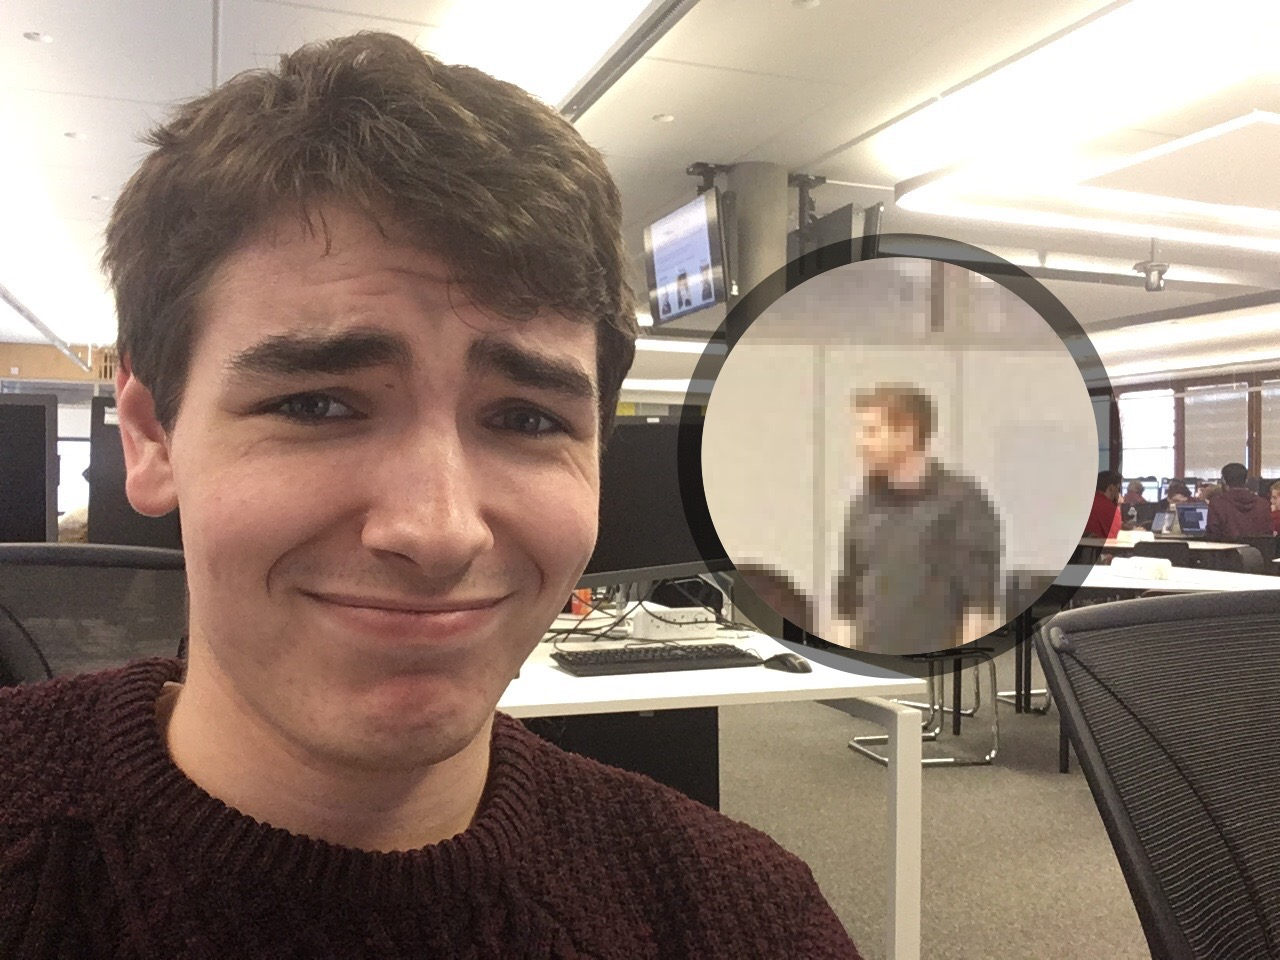
\includegraphics[width=0.5\textwidth]{max1.jpg}
\label{fig:selfie}
\end{figure}

My selfie with Max is in  Figure~\ref{fig:selfie}.

\subsection{What I have learned in this module}
I have learned and applied useful and practical skills that are sure to assist me in my future career as a computer scientist. Learning how to better communicate in teams of people I hadn't had the opportunity before and working together under pressure to produce good quality work that we are all proud of. I have learned the importance of communication and working under a leader, cooperating and collaborating whilst remaining calm and friendly with one another. Using diagrams and plans I am confident in methods used to plan and develop software and know that knowledge of these methods will help me through the actual development phase in the future.

